% AWS Lab_3.tex - AWS Lab 3 for Cloud Computing class (Spring 2015)
% Chanmann Lim - March 2015

\documentclass[a4paper]{article}

\usepackage[margin=1 in]{geometry}
\usepackage{listings}
\usepackage{graphicx}
\usepackage{float}

\begin{document}
\title{CS 7001-03: Report for AWS Lab 3 - Platform/Application Provisioning and Auto Scaling Adaptation}
\author{Chanmann Lim\\ 
	\texttt{cl9p8@mail.mail.missouri.edu}}
\date{March 31, 2015}
\maketitle

% ---------------------------------------- 1 ----------------------------------------
\paragraph{1. } Use \texttt{as-create-launch-config} command to create an AWS launch-configuration with options \texttt{--instance-type} set to 't1.micro', \texttt{--aws-credential-file} set to 'new-cf', \texttt{--image-id} set to 'ami-aa0237c2', \texttt{--key} set to 'new-key', \texttt{--group} set to 'new-group' and \texttt{--launch-config} set to 'new-lc':

\begin{verbatim}
# as-create-launch-config      \
  --instance-type t1.micro     \
  --aws-credential-file new-cf \
  --image-id ami-aa0237c2      \
  --key new-key                \
  --group new-group            \
  --launch-config new-lc
\end{verbatim}
Where 'ami-aa0237c2' is the custom AMI created from an instance of type 't1.micro'.

% ---------------------------------------- 2 ----------------------------------------
\paragraph{2. } Use \texttt{as-create-auto-scaling-group} command to create an auto scaling group and pass the name 'new-asg' as its argument along with options \texttt{--aws-credential-file} set to 'new-cf', \texttt{--availability-zones} set to 'us-east-1b', \texttt{--launch-configuration} set to 'new-lc', \texttt{--load-balancers} set to 'ELB', \texttt{--max-size} set to '5' and \texttt{--min-size} set to '1':

\begin{verbatim}
# as-create-auto-scaling-group new-asg \
  --aws-credential-file new-cf         \
  --availability-zones us-east-1b      \
  --launch-configuration new-lc        \
  --load-balancers ELB                 \
  --max-size 5                         \
  --min-size 1
\end{verbatim}
Where 'ELB' is an already created load balancer.

% ---------------------------------------- 3 ----------------------------------------
\paragraph{3. } Use \texttt{as-put-scaling-policy} command to create or update auto scaling policy and pass the name 'scale-up-policy' as its argument along with options \texttt{--auto-scaling-group} set to 'new-asg', \texttt{--adjustment=2} to scale up two instances, \texttt{--type} set to 'ChangeInCapacity', and \texttt{--cooldown} set to '240' for re-evaluating interval in seconds:

\begin{verbatim}
# as-put-scaling-policy scale-up-policy \
  --auto-scaling-group new-asg \
  --adjustment=2 \
  --type ChangeInCapacity \
  --cooldown 240
\end{verbatim}

% ---------------------------------------- 4 ----------------------------------------
\paragraph{4. } We should use Amazon CloudWatch to create an Alarm with 'new-asg' CPUUtilization metric to measure the computing resources then define threshold condition(e.g. CPUUtilization \textgreater= 50) and to trigger the policy we need to add AutoScaling Action then set \textbf{Whenever this alarm}: 'State is ALARM', \textbf{From the group}: 'new-asg', and \textbf{Take this action}: 'scale-up-policy'.

% ---------------------------------------- 5 ----------------------------------------
\paragraph{5. } The screenshots taken in Steps 3.5.3 and 3.5.4:
\begin{figure}[H]
  \centering
    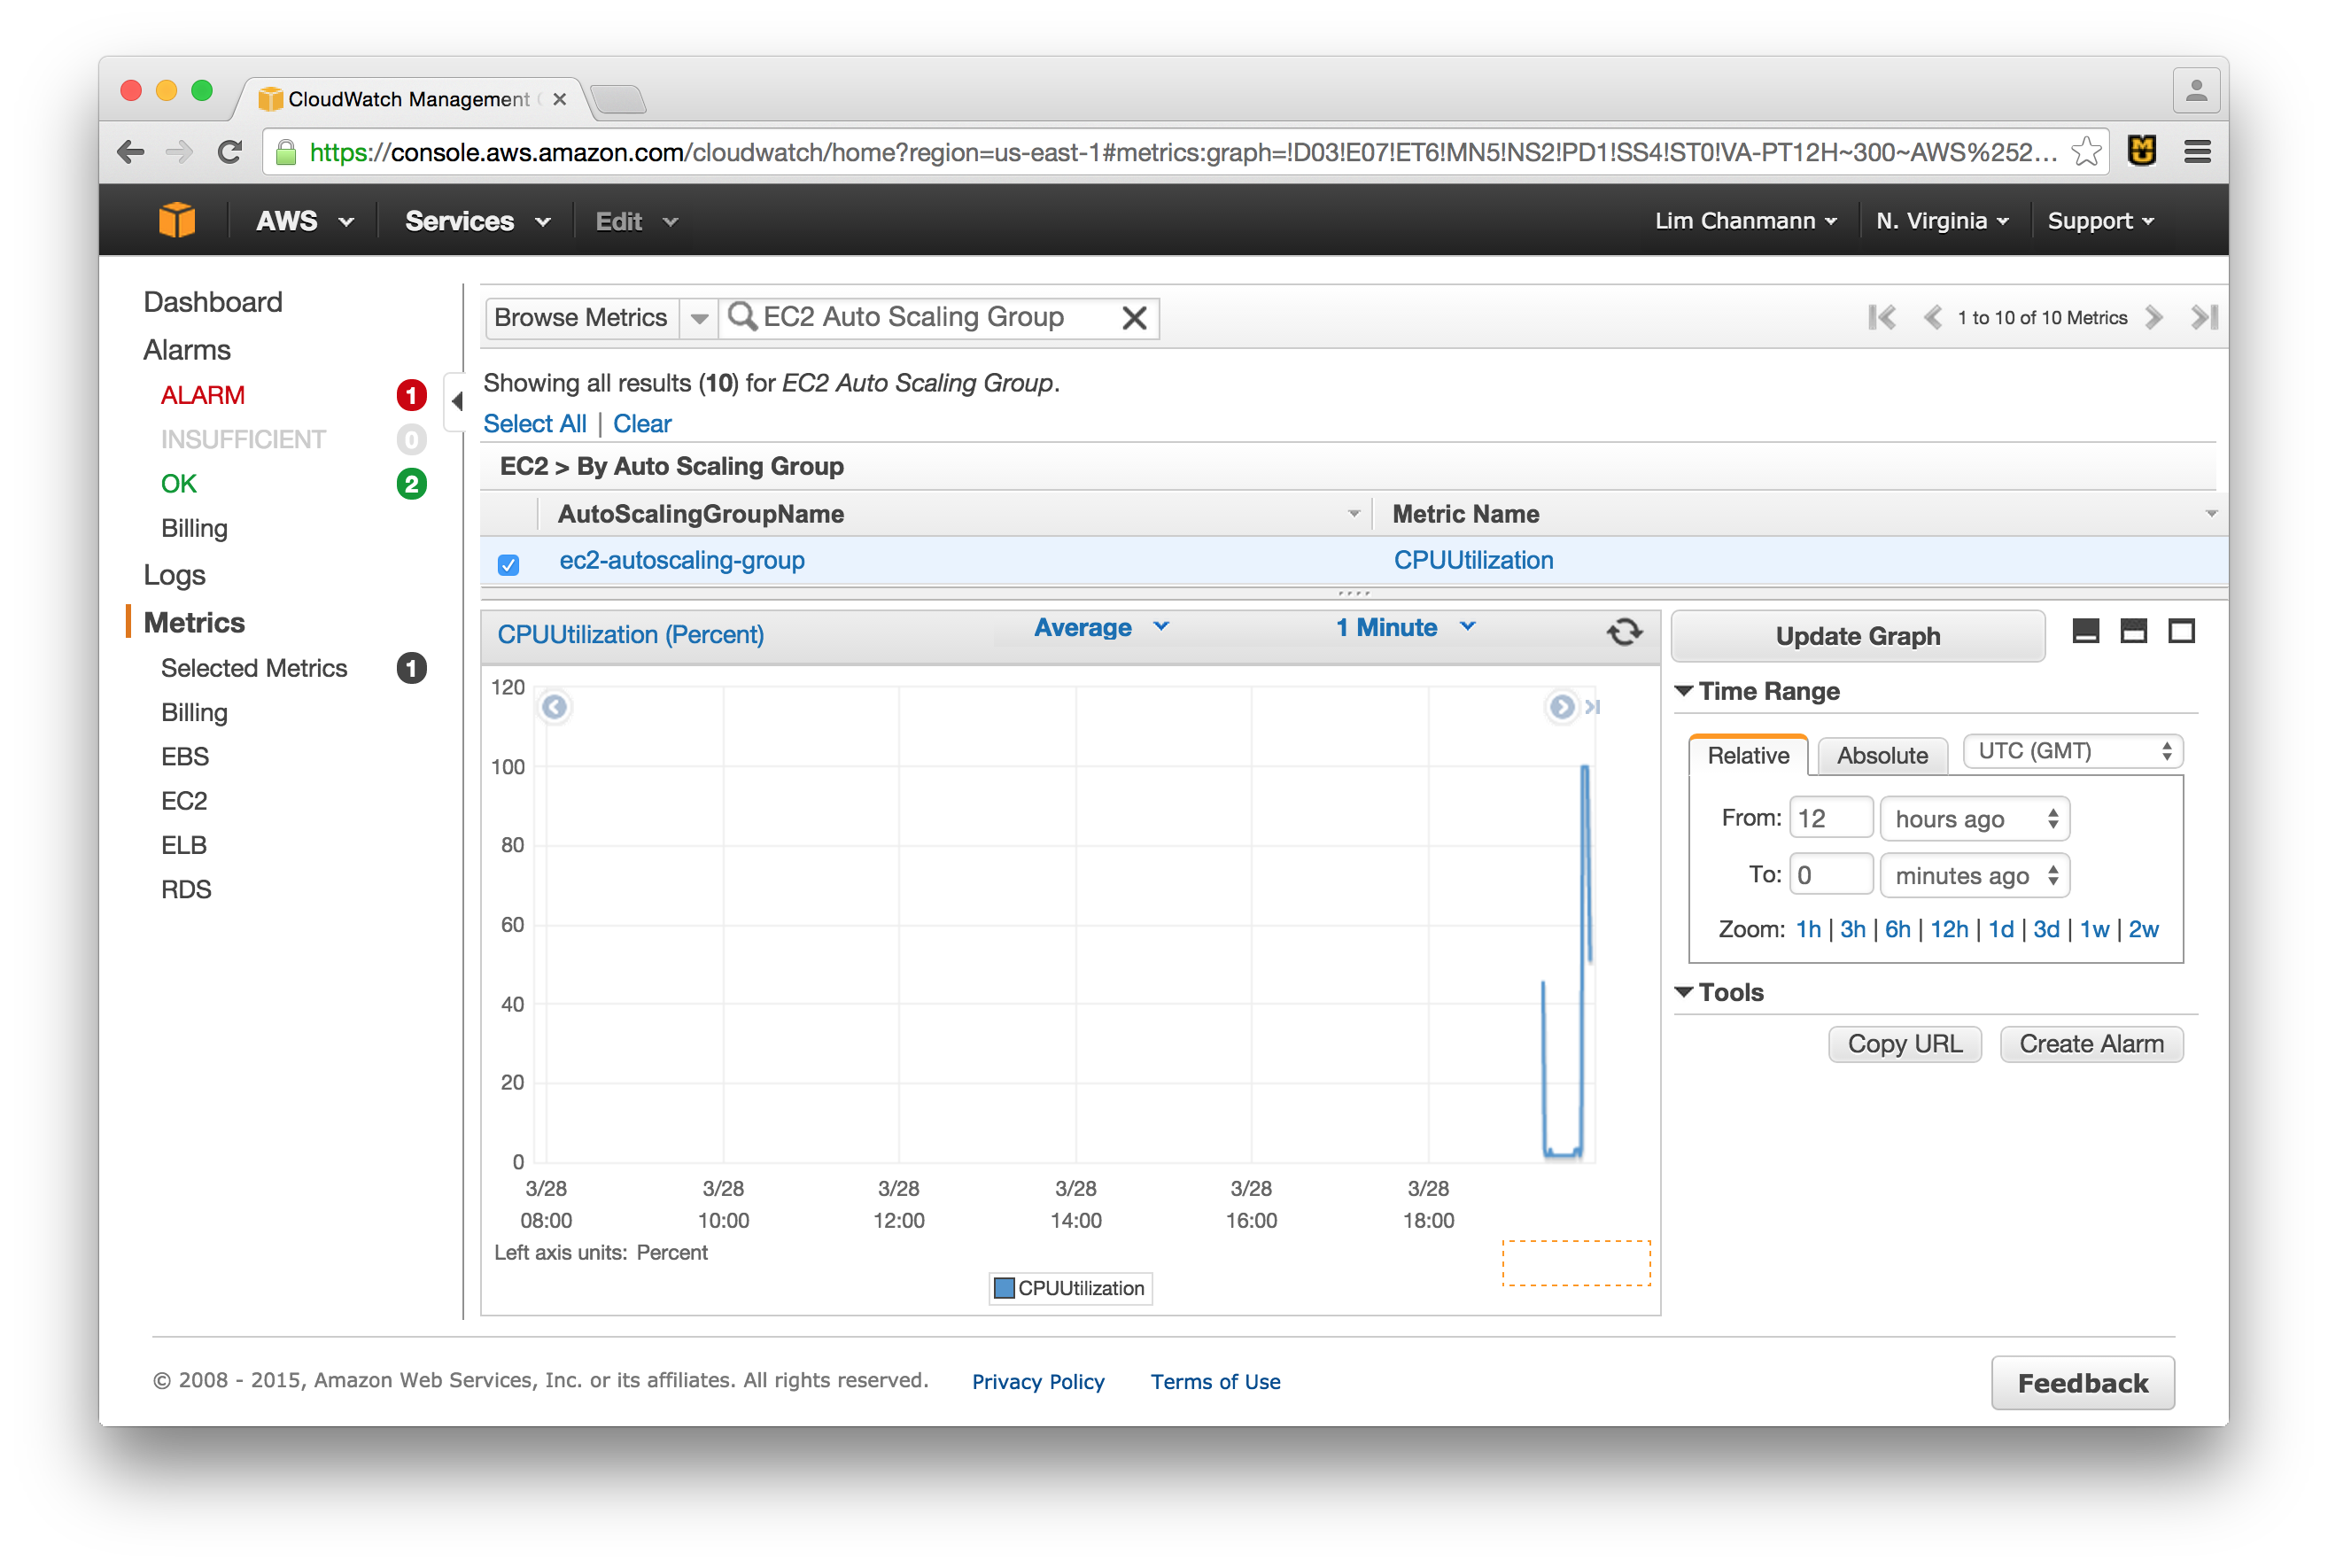
\includegraphics[scale=.34]{step_3_5_3.png}
  \caption{CPUUtilization metric during Apache Server benchmarking}
\end{figure}
\begin{figure}[H]
  \centering
    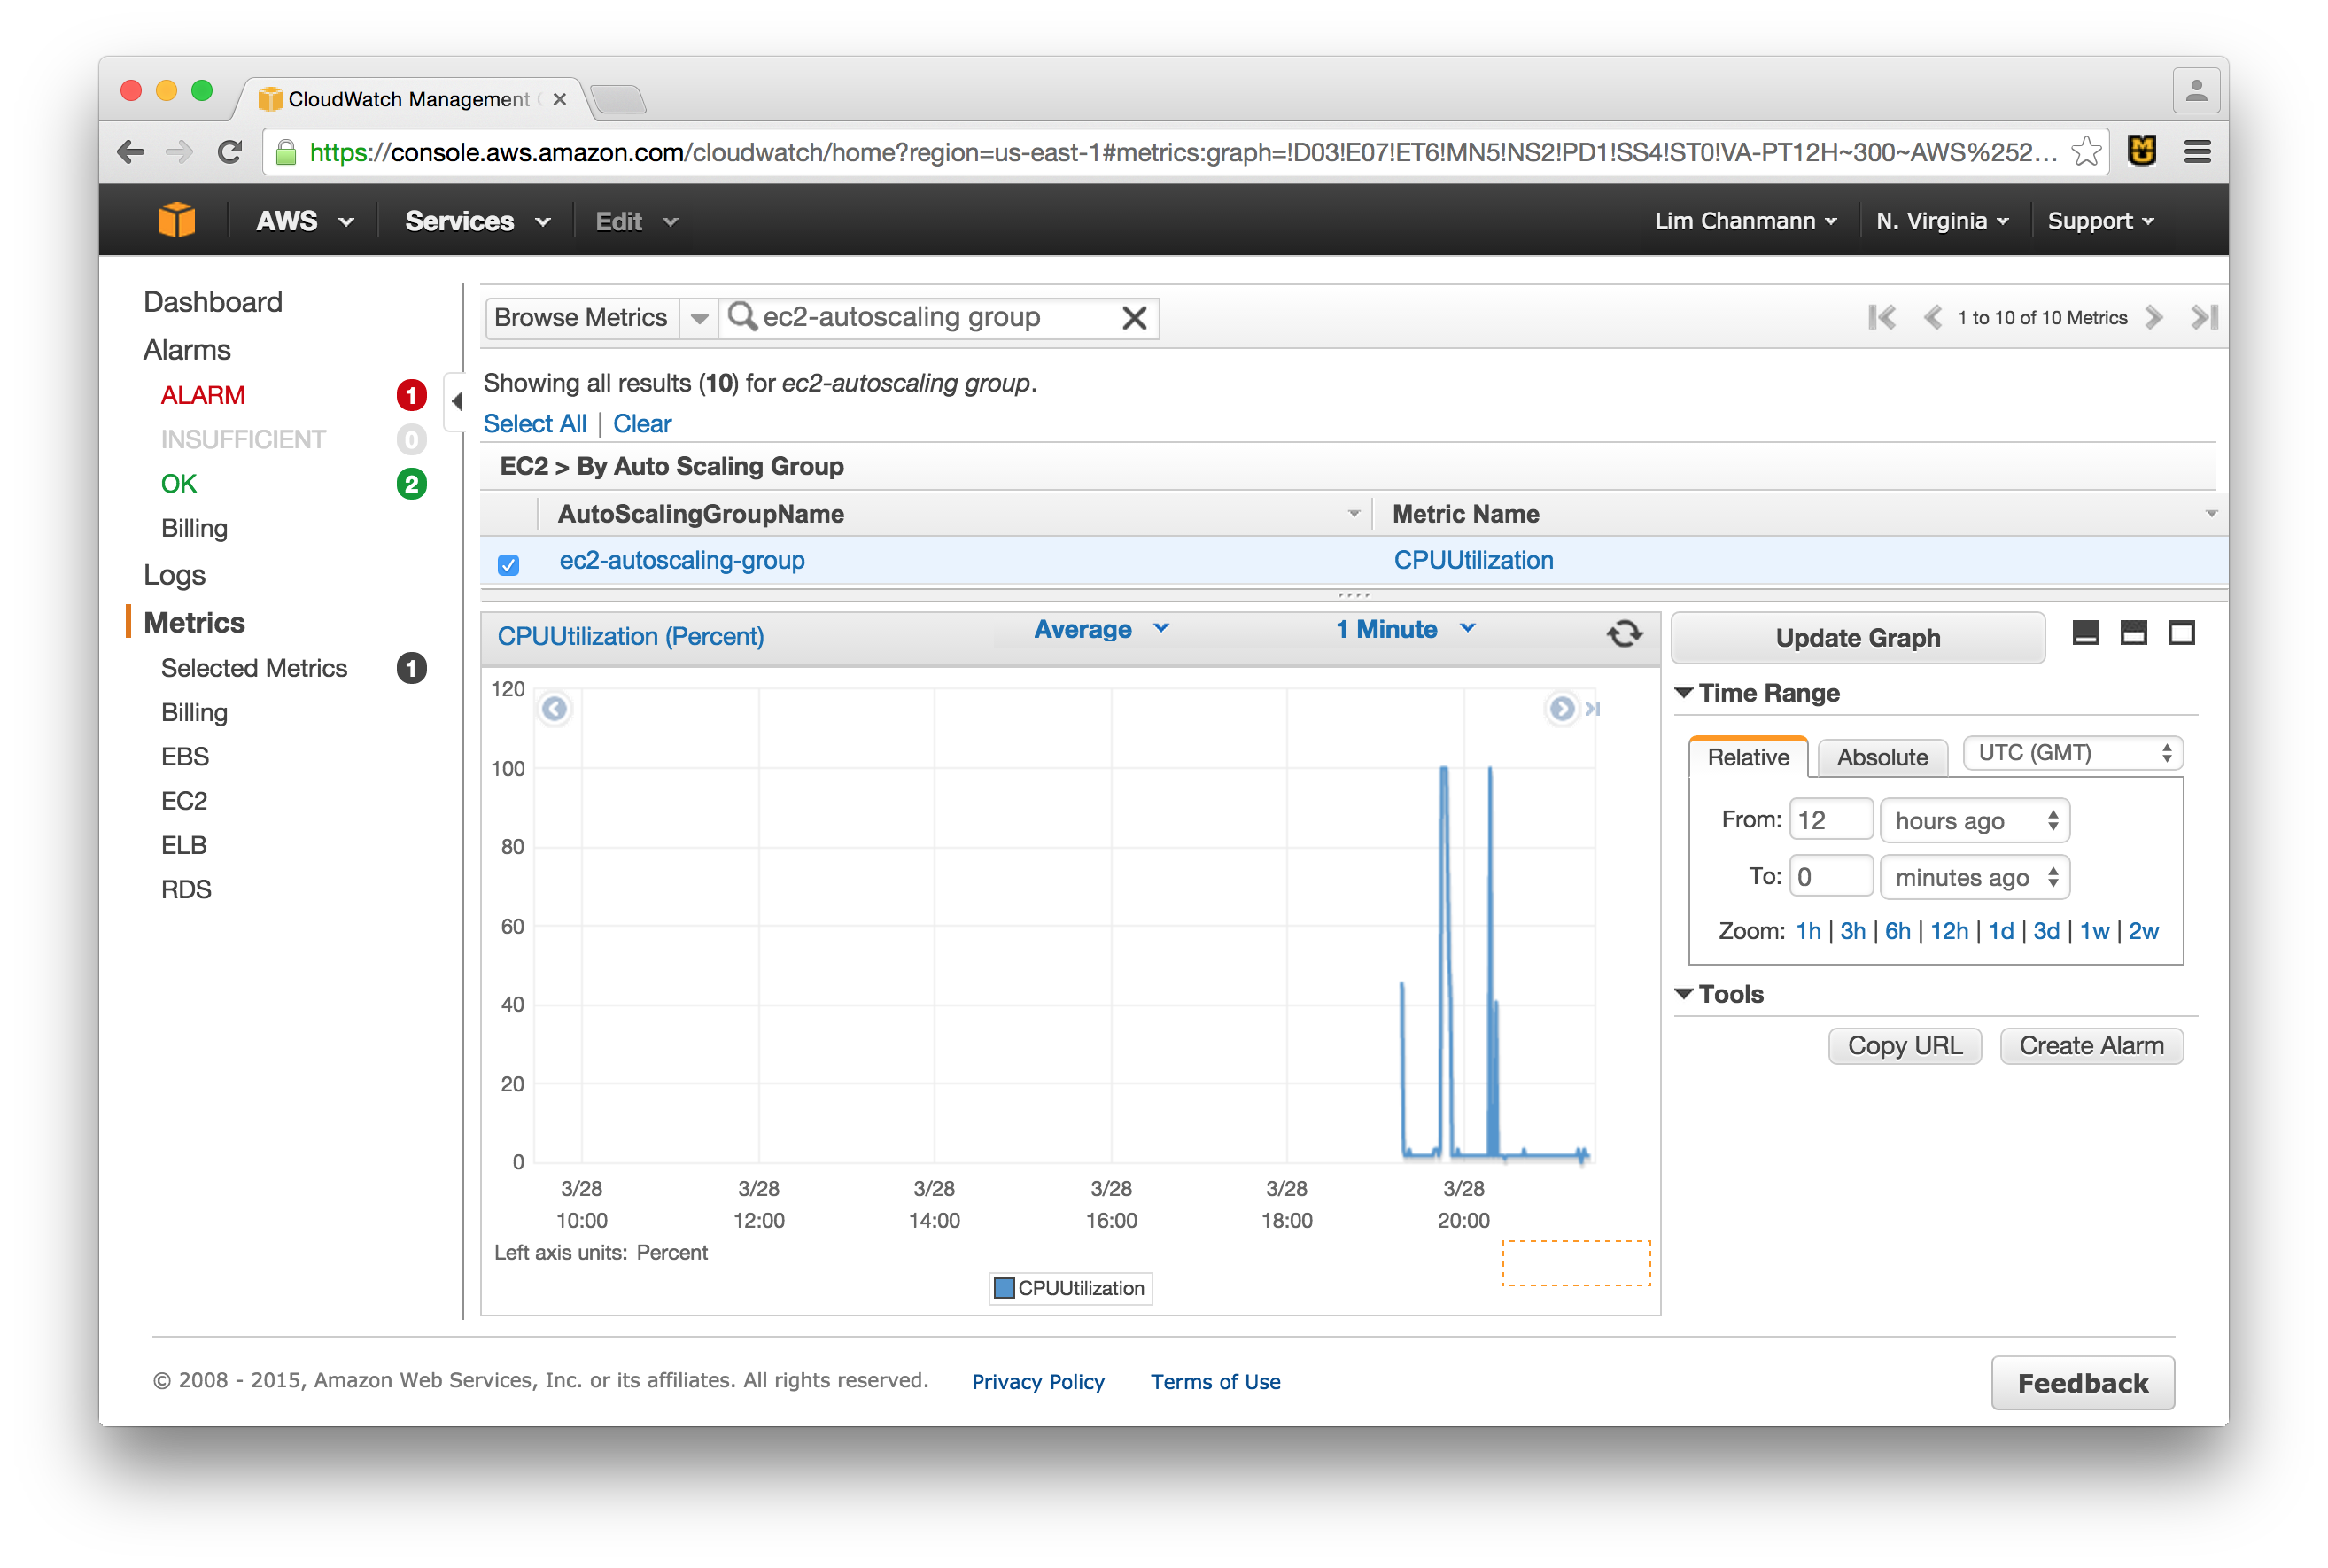
\includegraphics[scale=.34]{step_3_5_4.png}
  \caption{CPUUtilization metric after stopping benchmarking}
\end{figure}

% ---------------------------------------- 6 ----------------------------------------
%\paragraph{6. } Send an email to T.A Amit
%(ar442@mail.missouri.edu) with subject as "AWS" and a link to your load balancer in the body of your email. Once your grade will be posted on Blackboard you can execute the following commands.

\end{document}